\section*{Trifocal Tensor}
The Trifocal Tensor is a $3 \times 3 \times 3$ array of numbers that incorporates all projective geometric relationships among three views. It relates the coordinates of corresponding points or lines in three views, being independent of the scene structure and depending only on the relative motion among the three views and their intrinsic calibration parameters. Hence, the trifocal tensor can be considered as the generalization of the fundamental matrix in three views. It can also be seen as a collection of three rank-two $3 \times 3$ matrices $T_1, T_2, T_3$.
$\mathcal{T}_{i}^{jk}$ 

The geometric basis for the trifocal tensor can be deduced from the incidence relationship of three corresponding lines. We start by supposing a line 3-space is imaged in three views as in fig. \ref{fig:threeviews}. The planes back-projected from the lines in each view must all meet in a single line in space, the 3D line that projects to the mated line in the three images. Since in general three arbitrary planes in space do not meet in a single line, this geometric incidence condition provides a genuine constraint on sets of corresponding lines. 

\begin{figure}[ht!]
  \centering
  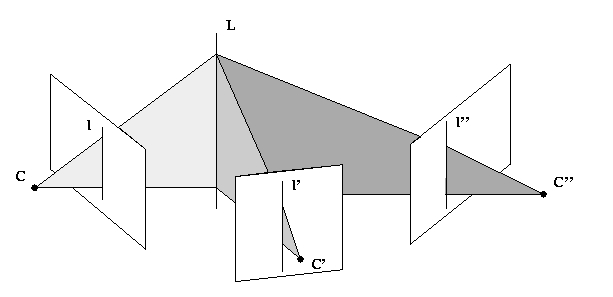
\includegraphics[width=100mm]{figures/threeviews.jpg}
  \caption{}
  \label{fig:threeviews}
\end{figure}

Let $ l_i \leftrightarrow l^{\prime}_i \leftrightarrow l^{\prime \prime}_i $ be the set of corresponding lines of $L$. Let the camera matrices for the three views be $P =  \begin{bmatrix} I \mid 0 \end{bmatrix}$, $P^{\prime} = \begin{bmatrix} A \mid a_{4} \end{bmatrix}$, $P^{\prime \prime} = \begin{bmatrix} B \mid b_{4} \end{bmatrix}$, where $A$ and $B$ are $3 \times 3$ matrices, and the vectors $a_i$ and $b_i$ are the \texttt{i}-th columns of the respective camera matrices for $i = 1,\dotsb,4$. $A$ and $B$ are the homographies from the first to the second and third cameras respectively. Due to our choice for the first camera matrix, $a_4$ and $b_4$ are consequently the epipoles of the first camera in views two and three respectively.
 \begin{align*}
  a_4 &= e^{\prime} = P^{\prime}C  & b_4 &= e^{\prime \prime}  = P^{\prime \prime}C
 \end{align*}

Each image line back-projects to a plane as shown in fig \ref{fig:threeviews}. These planes are 
\begin{align*}
\pi &= P^{T}l = \begin{pmatrix} l \\ 0 \end{pmatrix}  & \pi^{\prime} &= P^{\prime T}l^{\prime} = \begin{pmatrix} A^{T}l^{\prime} \\ a^{T}_{4}l^{\prime} \end{pmatrix} & \pi^{\prime \prime} &= P^{\prime \prime T}l^{\prime \prime} = \begin{pmatrix} B^{T}l^{\prime \prime} \\ b^{T}_{4}l^{\prime \prime} \end{pmatrix}
\end{align*}

The intersection constraint of the three planes in the common line in 3-space can be expressed algebraically by the requirement that the $4 \times 3$ matrix $ M = \begin{bmatrix} \pi & \pi^{\prime} & \pi^{\prime \prime} \end{bmatrix}$ has rank $2$. Points on the line of intersection may be represented as $X = \alpha X_1 + \beta X_2$, with $X_1$ and $X_2$ linearly independent. Such points lie on all three planes and so $\pi^{T}X = \pi^{\prime T}X = \pi^{\prime \prime T}X = 0$. It follows that $M^{T}X = 0$. Consequently M has a 2-dimensional null-space since $M^{T}X_1 = 0$ and $M^{T}X_2 =0$.

Since the rank of $M$ is 2, there is a linear dependence between its columns $m_i$, such that.
\begin{gather*}
M = \begin{bmatrix} m_1, m_2,m_3 \end{bmatrix} = \begin{bmatrix} l & A^{T}l^{\prime} & B^{T}l^{\prime \prime} \\
  0 & a^{T}_{4}l^{\prime} & b^{T}_{4}l^{\prime \prime}
\end{bmatrix}\\
m_1 = \alpha m_2 + \beta m_3
\end{gather*}

From the 2nd row of $M$, $\alpha = k(b^{T}_4 l^{\prime \prime})$ and $\beta = -k(a^{T}_4 l^{\prime})$ for some scalar $k$. Applying this back to the 1st row get 
\begin{gather*}
l = (b^{T}_4 l^{\prime \prime })A^{T}l^{\prime} - (a^{T}_4 l^{\prime})B^{T}l^{\prime \prime}\\
l = (l^{\prime \prime T} b_{4})A^{T}l^{\prime} - (l^{\prime T} a_{4})B^{T}l^{\prime \prime}
\end{gather*}

The \texttt{i}-th coordinate $l_i$ of $l$ may be written as
\begin{gather*}
  l_i = l^{\prime \prime T} (b_{4}a^{T}_{i}) l^{\prime} - l^{\prime T}(a_{4}b^{T}_{i}) l^{\prime \prime}\\
  l_i = l^{\prime T} (a_{i}b^{T}_{4}) l^{\prime \prime} - l^{\prime T}(a_{4}b^{T}_{i}) l^{\prime \prime}
\end{gather*}

This relationship can be expressed with the permutation tensor such as
\begin{gather*}
  \mathcal{T}_{i} = a_{i}b^{T}_{4} - a_{4}b^{T}_{i}\\
  l_i = l^{\prime T} \mathcal{T}_{i} l^{\prime \prime}
\end{gather*}

$\mathcal{T}$ is then the trifocal tensor relating the 3 views together. It has 27 elements. There are 26 independent rations apart from the common overall scaling factor of the tensor. However, the tensor has only 18 independent degrees of freedom. Each of 3 camera matrices has 11 degrees of freedom which makes $33$ in total. However, $15$ degrees of freedom must be subtracted to account for the projective world frame, thus leaving 18 degrees of freedom.

\begin{figure}[ht!]
  \centering
  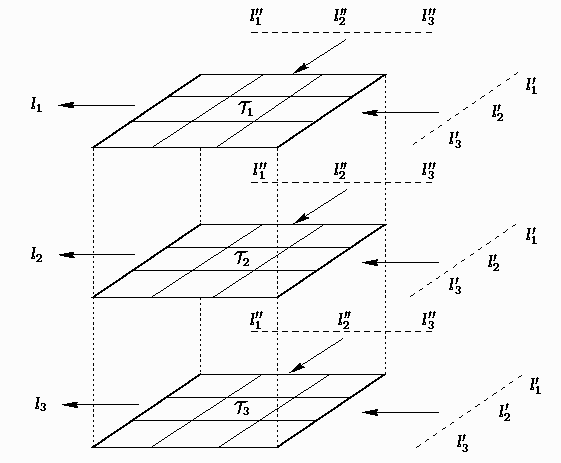
\includegraphics[width=100mm]{figures/trifocaltensor.png}
  \caption{\textbf{A 3D representation of the trifocal tensor}  $l_{i} = l_{j}^{\prime} l_{k}^{\prime \prime} \mathcal{T}_{i}^{jk}$ }
  \label{fig:trifocaltensor}
\end{figure}

A point $x$ on the line $l$ must satisfy $x^{T}l = \sum_{i} x^{i}l_{i} = 0$. Since $l_i = l^{\prime T} \mathcal{T}_{i} l^{\prime \prime}$, this may be written as
$
l^{\prime T}(\sum_{i} x^{i}\mathcal{T}_{i}) l^{\prime \prime} = 0
$
which means that there exists a 3D point $X$ mapping to $x$ in the first image, and to points on the lines $l^{\prime}$ and $l^{\prime \prime}$ in the second and third images. It's the incidence relationship that holds point-line-line correspondence.

To develop the point-point-point correspondence relationship, we can explore the homography map between the points on first and third images given by $x^{\prime \prime} = Hx$ and $l = H^{T}l^{\prime \prime}$. Thus we get
$$
  h_i = \mathcal{T}^{T}_{i}l^{\prime}
$$
Similarly, the homography from the first to the second views 
$$
  h_i = \mathcal{T}_{i}l^{\prime \prime}
$$

Using these results back to our point-line-line correspondence relation, 
\begin{gather*}
  x^{\prime \prime} = (\sum_{i} x^{i}\mathcal{T}^{T}_{i}) l^{\prime}
  x^{\prime \prime T}[x^{\prime \prime}]_{\times} = l^{\prime T} (\sum_{i} x^{i}\mathcal{T}_{i})[x^{\prime \prime}]_{\times} = 0^{T}
\end{gather*}

The line $l^{\prime}$ passes through $x^{\prime}$ may be written as $l^{\prime} = [x^{\prime}]_{\times}y^{\prime}$ for some point $y^{\prime}$ on $l^{\prime}$. Then
$$
  y^{\prime T} [x^{\prime}]_{times} (\sum_{i} x^{i}\mathcal{T}_{i})[x^{\prime \prime}]_{\times} = 0^{T}
$$

This relation holds true for all lines $l^{\prime}$ through $x^{\prime}$ and so is independent of $y^{\prime}$, hence this relation can be written as
$$
[x^{\prime}]_{times} (\sum_{i} x^{i}\mathcal{T}_{i})[x^{\prime \prime}]_{\times} = 0_{3\times 3}
$$
which expresses the point-point-point coincidence relationship required. Expressing this relation in proper tensor notation is then given by
$$
x^{i}(x^{\prime j} \epsilon_{jpr})(x^{\prime \prime k} \epsilon_{kqs})\mathcal{T}^{pq}_{i} = 0_{rs}
$$

\section*{Coefficients of the Trifocal Tensor}
To compute the relation between the coefficients of the trifocal tensor and the Projective matrices, first we write the Tensor relation formulated previously with the proper tensor notation as follows
$$
\mathcal{T}^{kl}_{j} = a^{k}_{j}b^{l}_{4} - a^{k}_{4}b^{l}_{j}
$$

For the sake of maintaining the Visual Servoing convention, we omit the use of $i$ as an index for the tensor relation. The letter $i$ further on will be indicating the initial view in the control system. The Camera positions are then written as $C^*,C_c,C_i$ for the desired, current, and initial camera positions respectively. The same may also be done for the projection matrices, and instead of using the matrices $A,B$ to express the homography between the first and second or third views, we will use the standard notation from Visual Servoing with the corresponding Rotation matrices $^{c^*}R_c, ^{c^*}R_i$ respectively.

\begin{align*}
  C &\Rightarrow C^* \text{  Desired camera position} \\
  C' &\Rightarrow C_c \text{  Current camera position} \\
  C^{''} &\Rightarrow C_i \text{  Initial camera position} \\
\end{align*}
\begin{gather*}
  P_d = P = [I | 0]\\
  P_c = P^{\prime} = [A | a_4] : ^{c^*}{\bf M}_c = [ ^{c^*}{\bf R}_c | ^{c^*}{\bf t}_c ]\\
  P_i = P^{\prime \prime} = [B | b_4] : ^{c^*}{\bf M}_i = [ ^{c^*}{\bf R}_i | ^{c^*}{\bf t}_i ]
\end{gather*}

The Tensor relation can then be expressed as follows 
$$
\mathcal{T}^{kl}_{j} = \tensor[^{c^*}]{R}{_{c}_{j}^{k}} \times \tensor[^{c^*}]{t}{_{i}^{l}} - \tensor[^{c^*}]{t}{_{c}^{k}} \times \tensor[^{c^*}]{R}{_{i}_{j}^{l}}
$$

Expanding this relation further to compute the tensor coefficients is straight forward, expanding for values of $j,k,l$ we get the following tensor coefficients:
\begin{gather*}
  \mathcal{T}^{11}_{1} = \tensor[^{c^*}]{R}{_{c}_{1}^{1}} \times \tensor[^{c^*}]{t}{_{i}^{1}} - \tensor[^{c^*}]{t}{_{c}^{1}} \times \tensor[^{c^*}]{R}{_{i}_{1}^{1}}\\
  \mathcal{T}^{12}_{1} = \tensor[^{c^*}]{R}{_{c}_{1}^{1}} \times \tensor[^{c^*}]{t}{_{i}^{2}} - \tensor[^{c^*}]{t}{_{c}^{1}} \times \tensor[^{c^*}]{R}{_{i}_{1}^{2}}\\
  \mathcal{T}^{13}_{1} = \tensor[^{c^*}]{R}{_{c}_{1}^{1}} \times \tensor[^{c^*}]{t}{_{i}^{3}} - \tensor[^{c^*}]{t}{_{c}^{1}} \times \tensor[^{c^*}]{R}{_{i}_{1}^{3}}\\
  \mathcal{T}^{21}_{1} = \tensor[^{c^*}]{R}{_{c}_{1}^{2}} \times \tensor[^{c^*}]{t}{_{i}^{1}} - \tensor[^{c^*}]{t}{_{c}^{2}} \times \tensor[^{c^*}]{R}{_{i}_{1}^{1}}\\
  \mathcal{T}^{22}_{1} = \tensor[^{c^*}]{R}{_{c}_{1}^{2}} \times \tensor[^{c^*}]{t}{_{i}^{2}} - \tensor[^{c^*}]{t}{_{c}^{2}} \times \tensor[^{c^*}]{R}{_{i}_{1}^{2}}\\
  \mathcal{T}^{23}_{1} = \tensor[^{c^*}]{R}{_{c}_{1}^{2}} \times \tensor[^{c^*}]{t}{_{i}^{3}} - \tensor[^{c^*}]{t}{_{c}^{2}} \times \tensor[^{c^*}]{R}{_{i}_{1}^{3}}\\
  \mathcal{T}^{31}_{1} = \tensor[^{c^*}]{R}{_{c}_{1}^{3}} \times \tensor[^{c^*}]{t}{_{i}^{1}} - \tensor[^{c^*}]{t}{_{c}^{3}} \times \tensor[^{c^*}]{R}{_{i}_{1}^{1}}\\
  \mathcal{T}^{32}_{1} = \tensor[^{c^*}]{R}{_{c}_{1}^{3}} \times \tensor[^{c^*}]{t}{_{i}^{2}} - \tensor[^{c^*}]{t}{_{c}^{3}} \times \tensor[^{c^*}]{R}{_{i}_{1}^{2}}\\
  \mathcal{T}^{33}_{1} = \tensor[^{c^*}]{R}{_{c}_{1}^{3}} \times \tensor[^{c^*}]{t}{_{i}^{3}} - \tensor[^{c^*}]{t}{_{c}^{3}} \times \tensor[^{c^*}]{R}{_{i}_{1}^{3}}\\
  \mathcal{T}^{11}_{2} = \tensor[^{c^*}]{R}{_{c}_{2}^{1}} \times \tensor[^{c^*}]{t}{_{i}^{1}} - \tensor[^{c^*}]{t}{_{c}^{1}} \times \tensor[^{c^*}]{R}{_{i}_{2}^{1}}\\
  \mathcal{T}^{12}_{2} = \tensor[^{c^*}]{R}{_{c}_{2}^{1}} \times \tensor[^{c^*}]{t}{_{i}^{2}} - \tensor[^{c^*}]{t}{_{c}^{1}} \times \tensor[^{c^*}]{R}{_{i}_{2}^{2}}\\
  \mathcal{T}^{13}_{2} = \tensor[^{c^*}]{R}{_{c}_{2}^{1}} \times \tensor[^{c^*}]{t}{_{i}^{3}} - \tensor[^{c^*}]{t}{_{c}^{1}} \times \tensor[^{c^*}]{R}{_{i}_{2}^{3}}\\
  \mathcal{T}^{21}_{2} = \tensor[^{c^*}]{R}{_{c}_{2}^{2}} \times \tensor[^{c^*}]{t}{_{i}^{1}} - \tensor[^{c^*}]{t}{_{c}^{2}} \times \tensor[^{c^*}]{R}{_{i}_{2}^{1}}\\
  \mathcal{T}^{22}_{2} = \tensor[^{c^*}]{R}{_{c}_{2}^{2}} \times \tensor[^{c^*}]{t}{_{i}^{2}} - \tensor[^{c^*}]{t}{_{c}^{2}} \times \tensor[^{c^*}]{R}{_{i}_{2}^{2}}\\
  \mathcal{T}^{23}_{2} = \tensor[^{c^*}]{R}{_{c}_{2}^{2}} \times \tensor[^{c^*}]{t}{_{i}^{3}} - \tensor[^{c^*}]{t}{_{c}^{2}} \times \tensor[^{c^*}]{R}{_{i}_{2}^{3}}\\
  \mathcal{T}^{31}_{2} = \tensor[^{c^*}]{R}{_{c}_{2}^{3}} \times \tensor[^{c^*}]{t}{_{i}^{1}} - \tensor[^{c^*}]{t}{_{c}^{3}} \times \tensor[^{c^*}]{R}{_{i}_{2}^{1}}\\
  \mathcal{T}^{32}_{2} = \tensor[^{c^*}]{R}{_{c}_{2}^{3}} \times \tensor[^{c^*}]{t}{_{i}^{2}} - \tensor[^{c^*}]{t}{_{c}^{3}} \times \tensor[^{c^*}]{R}{_{i}_{2}^{2}}\\
  \mathcal{T}^{33}_{2} = \tensor[^{c^*}]{R}{_{c}_{2}^{3}} \times \tensor[^{c^*}]{t}{_{i}^{3}} - \tensor[^{c^*}]{t}{_{c}^{3}} \times \tensor[^{c^*}]{R}{_{i}_{2}^{3}}\\
  \mathcal{T}^{11}_{3} = \tensor[^{c^*}]{R}{_{c}_{3}^{1}} \times \tensor[^{c^*}]{t}{_{i}^{1}} - \tensor[^{c^*}]{t}{_{c}^{1}} \times \tensor[^{c^*}]{R}{_{i}_{3}^{1}}\\
  \mathcal{T}^{12}_{3} = \tensor[^{c^*}]{R}{_{c}_{3}^{1}} \times \tensor[^{c^*}]{t}{_{i}^{2}} - \tensor[^{c^*}]{t}{_{c}^{1}} \times \tensor[^{c^*}]{R}{_{i}_{3}^{2}}\\
  \mathcal{T}^{13}_{3} = \tensor[^{c^*}]{R}{_{c}_{3}^{1}} \times \tensor[^{c^*}]{t}{_{i}^{3}} - \tensor[^{c^*}]{t}{_{c}^{1}} \times \tensor[^{c^*}]{R}{_{i}_{3}^{3}}\\
  \mathcal{T}^{21}_{3} = \tensor[^{c^*}]{R}{_{c}_{3}^{2}} \times \tensor[^{c^*}]{t}{_{i}^{1}} - \tensor[^{c^*}]{t}{_{c}^{2}} \times \tensor[^{c^*}]{R}{_{i}_{3}^{1}}\\
  \mathcal{T}^{22}_{3} = \tensor[^{c^*}]{R}{_{c}_{3}^{2}} \times \tensor[^{c^*}]{t}{_{i}^{2}} - \tensor[^{c^*}]{t}{_{c}^{2}} \times \tensor[^{c^*}]{R}{_{i}_{3}^{2}}\\
  \mathcal{T}^{23}_{3} = \tensor[^{c^*}]{R}{_{c}_{3}^{2}} \times \tensor[^{c^*}]{t}{_{i}^{3}} - \tensor[^{c^*}]{t}{_{c}^{2}} \times \tensor[^{c^*}]{R}{_{i}_{3}^{3}}\\
  \mathcal{T}^{31}_{3} = \tensor[^{c^*}]{R}{_{c}_{3}^{3}} \times \tensor[^{c^*}]{t}{_{i}^{1}} - \tensor[^{c^*}]{t}{_{c}^{3}} \times \tensor[^{c^*}]{R}{_{i}_{3}^{1}}\\
  \mathcal{T}^{32}_{3} = \tensor[^{c^*}]{R}{_{c}_{3}^{3}} \times \tensor[^{c^*}]{t}{_{i}^{2}} - \tensor[^{c^*}]{t}{_{c}^{3}} \times \tensor[^{c^*}]{R}{_{i}_{3}^{2}}\\
  \mathcal{T}^{33}_{3} = \tensor[^{c^*}]{R}{_{c}_{3}^{3}} \times \tensor[^{c^*}]{t}{_{i}^{3}} - \tensor[^{c^*}]{t}{_{c}^{3}} \times \tensor[^{c^*}]{R}{_{i}_{3}^{3}}
\end{gather*}
